\renewcommand{\theequation}{\theenumi}
\begin{enumerate}[label=\thesection.\arabic*.,ref=\thesection.\theenumi]
\numberwithin{equation}{enumi}

\item A point $\vec{c}$ lying on the line 
\begin{align}
\myvec{a&b}\vec{x} = c
\end{align}
at a distance $\lambda$ from point $\vec{x}$ lying on the same line is given as
\begin{align}
\vec{c} = \vec{x} + \frac{\lambda}{\sqrt{a^2+b^2}}\myvec{b\\-a}
\\
\vec{c} = \vec{x} + \myvec{b\\-a}
For, \lambda={\sqrt{a^2+b^2}
\label{second_point}
\end{align}


\item Equation of y axis is 
\begin{align}
\myvec{1&0}\vec{x}=0
\label{eq:y_axis}
\end{align}
\item 
\begin{align}
\brak{a} \myvec{4&3}\vec{x}=12
\end{align}
The line meets y-axis at point $\vec{y_1}$ given using \ref{eq:y_axis} as,
\item 
\begin{align}
\myvec{4&3\\1&0}\vec{y_1} =\myvec{12\\0}
\\
\vec{y_1}={\myvec{4&3\\1&0}}^{-1}\myvec{12\\0}
\\
\vec{y_1}=\myvec{0\\4}
\end{align}
Another point $\vec{c_1}$ on the line is found using equation \ref{eq:second_point}
\begin{align}
\vec{c_1} = \vec{y_1} + \myvec{3\\-4}
\\
\implies \vec{c_1} = \myvec{3\\0}
\end{align}
\newline

\begin{align}
\brak{b}\myvec{2&5}\vec{x}=0
\end{align}
The line meets y-axis at point $\vec{y_2}$ given using \ref{eq:y_axis} as,
\item 
\begin{align}
\myvec{2&5\\1&0}\vec{y_1} =\myvec{0\\0}
\\
\vec{y_1}={\myvec{2&5\\1&0}}^{-1}\myvec{0\\0}
\\
\vec{y_1}=\myvec{0\\0}
\end{align}
Another point $\vec{c_2}$ on the line is found using equation \ref{eq:second_point}
\begin{align}
\vec{c_2} = \vec{y_2} + \myvec{5\\-2}
\\
\implies \vec{c_2} = \myvec{5\\-2}
\end{align}

\begin{align}
\brak{c}\myvec{0&3}\vec{x}=4
\end{align}
The line meets y-axis at point $\vec{y_2}$ given using \ref{eq:y_axis} as,
\item 
\begin{align}
\myvec{0&3\\1&0}\vec{y_1} =\myvec{4\\0}
\\
\vec{y_1}={\myvec{0&3\\1&0}}^{-1}\myvec{4\\0}
\\
\vec{y_1}=\myvec{0\\\frac{4}{3}}
\end{align}
Another point $\vec{c_2}$ on the line is found using equation \ref{eq:second_point}
\begin{align}
\vec{c_2} = \vec{y_2} + \myvec{3\\0}
\\
\implies \vec{c_2} = \myvec{3\\\frac{4}{3}}
\end{align}
The python code for the above problem , plotting the figure \ref{fig:three_lines} is available at 
\begin{lstlisting}
codes/line/pointonline2/pointonline.py
\end{lstlisting}
\begin{figure}[!ht]
\centering
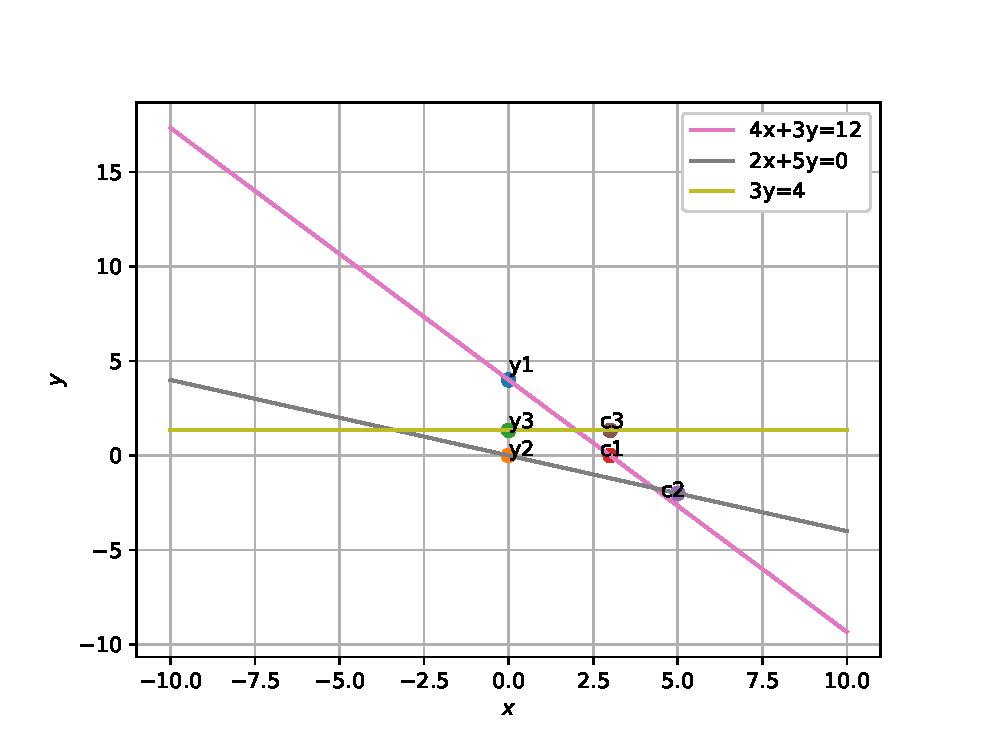
\includegraphics[width=\columnwidth]{./codes/line/pointonline2/pyfigs/pointonline.eps}
\caption{Plot of the three lines and the points on them }
\label{fig:three_lines}
\end{figure}

\end{enumerate}
